
\section{Series} While a sequence is a list of numbers, a series is a sum of a list of numbers.  That is, a sequence is a list of numbers with commas inbetween; a series is a list of numbers with plus signs inbetween.  We often use the very compact \emph{sigma notation} to represent series. 

\begin{definition}{Sigma Notation for Series}
If $a_n$ is a sequence and $j,k$ are both natural numbers, then we define the series:
$$\sum_{n=j}^k a_n =a_{j}+a_{j+1}+a_{j+2}+\cdots+a_{k}$$ That is, we add up all consecutive terms of the sequence $a_n$, starting at index $j$ and stopping at index $k$.
\end{definition}
Notice that the above summation has $k-j+1$ terms in it, not $k-j$ as one might quickly guess.  One way to see this is to rewrite the sum slightly as
$$a_{j}+a_{j+1}+a_{j+2}+\cdots+a_{k}=\underset{\text{One extra for term }0\ldots}{\underbrace{a_{j+0}}}+\underset{\text{\ldots then count terms }1,2,\ldots k}{\underbrace{a_{j+1}+a_{j+2}+\cdots+a_{k}}}.$$

This subtlety is often called an \emph{off by one error} or \emph{fencepost problem}, since one can view it as if the plus signs were sections of fence, and the terms in the sequence were posts holding up those sections.  To support $k-j$ sections of fence, we need $k-j+1$ posts, since each section has a post to the right of it, but the very first section of fence also has a post to the left which is not to the right of any section. 

If the starting index is greater than the stopping index, we consider the sum to be empty.  Since it has no terms, we define the total to be zero.  Thus, an \emph{empty sum} is the additive identity zero, just like an empty product is the multiplicative identity one.

The sequence $a_n$ that is being totaled is called the \emph{summand}, much as the function $f(x)$ is referred to as the integrand in the expression $\int f(x) \dif x$.

\begin{example}{Evaluating a Summation}
Consider the sum of all even numbers between six and fourteen.  Of course we don't need sigma notation to evaluate such a sum, but just for proof of  concept, let's write this sum in sigma notation, expand, and evaluate. 
\begin{itemize}
\item First we discuss the summand.  The sequence of all even numbers has the explicit formula $a_n=2n$, so $2n$ will be our summand.
\item We want the first term to be six, so we set $n=3$ as the starting index. 
\item We want the last term to be fourteen, so we set $n=7$ as the stopping index.

\end{itemize}

Thus our summation is 
\begin{align*}
\sum_{n=3}^{7}2n &= \underset{n=3}{\underbrace{6}}+\underset{n=4}{\underbrace{8}}+\underset{n=5}{\underbrace{10}}+\underset{n=6}{\underbrace{12}}+\underset{n=7}{\underbrace{14}} \\
 &= 60.
\end{align*}

\end{example}

\begin{exercise}{Not Crashing Into That Extra Fencepost \Coffeecup}
The summation in the above example has starting index 3 and stopping index 7.  So, does the sum have $7-3=4$ terms, or does it have $7-3+1=5$ terms?

\end{exercise}


\begin{exercise}{Sigma Notation \Coffeecup}
Evaluate the following sums:
\begin{itemize}
\item $\sum\limits_{n=0}^{3} 2n $
\item $\sum\limits_{n=0}^{3} (-1)^nn^2 $
\item $\sum\limits_{n=0}^{3} 2^n $
\end{itemize}
\AnswerKeyEntry{The totals are 12, -6, and 15.}
\end{exercise}

\begin{exercise}{Properties of Summations \Coffeecup \Coffeecup \Coffeecup }
Let $c$ be an arbitrary real number, $j$ and $k$ natural numbers with $j<k$, and $a_n$ and $b_n$ be arbitrary sequences.  For each of the following properties, explain why it is true, or come up with a counterexample that shows it is not.
\begin{itemize}
\item $\sum\limits_{n=j}^{k} c\cdot a_n=c\sum\limits_{n=j}^{k} a_n $
\vspace*{.5in}
\item $\sum\limits_{n=j}^{k} \left( a_n+b_n\right) =\left(\sum\limits_{n=j}^{k}  a_n\right) +\left( \sum\limits_{n=j}^{k} b_n\right)$
\vspace*{.4in}
\item $\sum\limits_{n=j}^{k} \left( a_n\cdot b_n\right) =\left(\sum\limits_{n=j}^{k}  a_n\right) \cdot\left( \sum\limits_{n=j}^{k} b_n\right) $
\vspace*{.4in}
\item  $\sum\limits_{n=0}^{k}  a_n =\sum\limits_{n=1}^{k+1}  a_{n-1}$
\vspace*{.4in}
\item  $\sum\limits_{n=0}^{k}  c =ck$
\vspace*{.4in}
\item  $\sum\limits_{n=1}^{k}  c =ck$
\vspace*{.4in}
\end{itemize}
\AnswerKeyEntry{It is easiest to just expand the sums on both sides and see what the terms look like.  For example, in the first case the left-hand side is $\left(ca_j+ca_{j+1}+\cdots+ca_k\right)$, whereas the right-hand side is $c\left(a_j+a_{j+1}+\cdots+a_k\right)$.  These two expressions are equal, because we can factor the $c$ out of the left-hand side to produce the right-hand side.  For the last two summations, think about our discussion of fencepost problems above!}
\end{exercise}

\section{Arithmetic Series} If the \arithmeticsequence{summand} $a_n$ is an arithmetic sequence, the summation is called an \emph{arithmetic series}.  In this case, we have a nice \arithmeticseries{formula} for the sum!  

\begin{theorem}{Arithmetic Series Formula}  Let $a_n$ be an \series{arithmetic} sequence with initial term $a_0$ and common difference $d$.  Then the following sum has closed form $$\sum_{n=0}^N a_n = \left(N+1\right)\cdot\frac{a_0+\left(a_0+Nd\right)}{2}. $$
\end{theorem}

A nice short way to state the \area{arithmetic series formula} is as follows: 
\begin{center}
\emph{The sum of an arithmetic series is equal to the number of terms times the average of the first term and the last term.}\end{center}

\begin{exercise}{Lining Up the Formal and the Informal \Coffeecup}
In the more formal statement of the arithmetic series formula, what expression represents... 
\begin{itemize}
\item ...``number of terms"?
\item ...``first term"?
\item ...``last term"?
\item ...``average"?
\end{itemize}
\end{exercise}

\begin{exercise}{A \arithmeticseries{Visual Argument} for the Arithmetic Series Formula \Coffeecup \Coffeecup \Coffeecup}
Here we draw a diagram to show why the Arithmetic Series Formula works.  
Consider the arithmetic sum $$\left(a_0\right)+\left(a_0+d\right)+\left(a_0+2d\right)+\cdots+\left(a_0+Nd\right).$$
\begin{itemize}

\item For each term in the sum, we draw a corresponding rectangle.  Specifically, a one by $a_0$ rectangle represents the first term, a one by $a_0+d$ rectangle represents the second term, and so on.  These rectangles are stacked in order in the first quadrant, next to each other on the $x$-axis, with sides of width one all on the $x$-axis.  Explain why the area of the region is equal to the sum. \vspace*{1in}

	\begin{center}
		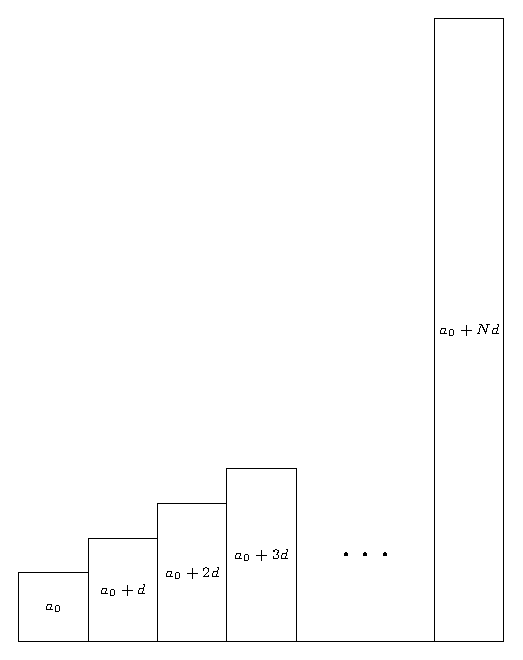
\includegraphics[width=200pt]{ChapterSeqSer/Figures/arithmetic.eps}
	\end{center}

\item Duplicate the entire region in the opposite order to build one giant rectangle.  Draw a one by $a_0 +Nd$ rectangle on top of the leftmost, then a one by $a_0+(N-1)d$ rectangle on top of the second, and so on until the last rectangle gets topped with a one by $a_0$ rectangle.  In this new giant rectangle that is formed...

\begin{itemize}
\item  ...what is the width?
\item ...what is the height?
\item ...what is the total area?
\end{itemize}

\item Explain why the total area of that rectangle must be exactly double the value of the arithmetic sum.  
\vspace*{.5in}
\item Divide the total area by two to arrive at the arithmetic series formula!
\vspace*{.5in}
\end{itemize}
\end{exercise}

Note that you have seen something similar in Calculus I in the context of evaluating Riemann Sums.  In particular, \arithmeticseries{Gauss's Formula} states $$ \sum_{n=1}^Nn=\frac{N\left(N+1\right)}{2}.$$

\begin{exercise}{Gauss's Formula as an Arithmetic Series \Coffeecup \Coffeecup}

Pretend for a second (or thirty) that you do not know Gauss's Formula.  Evaluate $\sum_{n=1}^Nn$ using the Arithmetic Series Formula.  Verify this produces the right-hand side of Gauss's Formula.  \AnswerKeyEntry{ In Gauss's formula, the first term $a_0$ and the common difference $d$ are both 1.  The number of terms is $N$.  Plugging these into the Arithmetic Series Formula will produce $N(N+1)/2$.}
\vspace*{1in}
\end{exercise}

\begin{example}{Adding Multiples of Six }
Suppose we wish to find the sum of all multiples of six between 1000 and 2000.  We notice that neither 1000 nor 2000 are divisible by six. However, multiples of six can never be too far away.  In particular, $1002=6\cdot167$ and $1998=6\cdot 333$.  Thus, the summation we wish to evaluate is $$1002+1008+1014+\cdots+1998 $$ which can also be written as $$6\cdot167+6\cdot168+6\cdot169+\cdots+6\cdot333. $$  From the above forms, we now have all the information we need to apply the Arithmetic Series Formula.
\begin{itemize}
\item First Term: $1002$
\item Last Term: $1998$
\item Number of Terms, Remembering the Fencepost: $333-167+1=167$
\end{itemize}
We now evaluate the summation using the Arithmetic Series Formula as follows: \begin{align*}
1002+1008+1014+\cdots+1998 &=\left(\text{Number of Terms}\right)\left(\text{Average of First and Last}\right)\\ 
&=\left(167\right)\left(\frac{1002+1998}{2}\right)\\
&=167\cdot 1500 \\
&=250,500.
\end{align*}
\end{example}

\begin{exercise}{Practice with Arithmetic Series \Coffeecup \Coffeecup}

\begin{itemize}

\item  Add up all the whole numbers from 1 to 1000 inclusive.

\vspace*{.6in}

\item Add up all the whole numbers from 1000 to 2000 inclusive.

\vspace*{.6in}

\item What is the sum of all multiples of seven between 1000 and 2000?

\vspace*{.6in}

\item Compute the following summation using the Arithmetic Series Formula: $$ \sum_{n=4}^{13} (3n-1).$$

\vspace*{.6in}

\end{itemize}

\AnswerKeyEntry{The totals are 500500, 1501500, 214214, and 245.}

\end{exercise}

\section{Geometric Series} If the summand $a_n$ is a \series{geometric} sequence, the summation is called an \emph{geometric series}.  In this case, we again have a nice formula for the sum!  

\begin{theorem}{\geometricseries{Finite} Geometric Series Formula}  Let $a_n$ be a geometric sequence with initial term $a_0$ and common ratio $r$.  Then the following sum has closed form $$\sum_{n=0}^N a_n = a_0\cdot\frac{1-r^{N+1}}{1-r}. $$
\end{theorem}

In words, you can state the geometric series formula as follows:
\begin{center}\emph{The sum of a geometric series is equal to the first term times one minus the common ratio raised to the number of terms, divided by one minus the common ratio.}\end{center}

\begin{exercise}{An Algebraic Argument for the Geometric Series Formula \Coffeecup \Coffeecup \Coffeecup}
Here we use algebra to demonstrate why the Geometric Series Formula is valid.  
Consider the following geometric series and call it $S$ for sum:  $$S=\left(a_0\right)+\left(a_0r\right)+\left(a_0r^2\right)+\cdots+\left(a_0r^N\right)$$
\begin{itemize}

\item Explain why the following equality holds:

$$ rS=\left(a_0r\right)+\left(a_0r^2\right)+\left(a_0r^3\right)+\cdots+\left(a_0r^{N+1}\right)$$

\item Subtract the two above equations.  Fill in the right hand side below.
$$S-rS=\hspace{3.5in} $$
\item Solve for $S$ in the equation above to construct the Geometric Series Formula!
\vspace*{.5in}
\end{itemize}
\end{exercise}

\begin{exercise}{Trying Out the Geometric Series Formula \Coffeecup }
Consider the summation $1+10+10^2+10^3+10^4+10^5. $
\begin{itemize}
\item Find the total by just doing the arithmetic.  Evaluate the powers of ten and then add them up. 

\vspace*{.5in}
\item Find the total by using the Geometric Series Formula.  Verify that your answers match! 

\vspace*{.5in}

\end{itemize}
\AnswerKeyEntry{The common ratio $r=10$.  The first term is 1.  The number of terms is 6.  Putting this all together in the Geometric Series Formula produces $1\cdot\frac{1-10^6}{1-10}=\frac{-99999}{-9}=11111.$}
\end{exercise}

\begin{exercise}{Powers of Two \Coffeecup \Coffeecup}
Consider the summation $1+2+2^2+2^3+2^4+2^5. $
\begin{itemize}
\item Find the total by just doing the arithmetic.  Evaluate the powers of two and then add them up. 

\vspace*{.5in}

\item Find the total by using the Geometric Series Formula.  Verify that your answers match! 

\vspace*{.5in}

\item Use the Geometric Series Formula to evaluate $$1+2+2^2+2^3+\cdots+2^N. $$

\vspace*{.5in}

\item Write in words the answer to the following: ``\emph{A finite sum of consecutive powers of two, starting at one, is equal to... }''
 
\vspace*{.5in}

\end{itemize}
\AnswerKeyEntry{A finite sum of consecutive powers of two, starting at one, is equal to one less than the next power of two.}
\end{exercise}


\begin{example}{Difference of Two Quartics Formula}  Here we show how the geometric series formula can be used to obtain a factorization formula!  In particular, let us evaluate the summation $$A^3+A^2B+AB^2+B^3.$$  We follow the little remark above, noting that the first term is $\left(A^3\right)$ and the common ratio is $\left(B/A\right)$.  We now evaluate the sum and then clean up the resulting compound fraction:
\begin{align*}
A^3+A^2B+AB^2+B^3&=A^3\frac{1-\left(\frac{B}{A}\right)^4}{1-\left(\frac{B}{A}\right)}\\
&=A^3\frac{A-B^4/A^3}{A-B}\\
&=\frac{A^4-B^4}{A-B}.\\
\end{align*} 

Multiplying both sides by $A-B$, we have the difference of two quartics factorization as follows: $$A^4-B^4=(A-B)\cdot\left(A^3+A^2B+AB^2+B^3\right).$$
\end{example}

\begin{exercise}{Difference of Two Cubes}
\begin{itemize}
\item In the same manner, use the geometric series formula to build the more familiar difference of two cubes formula: $$A^3-B^3=(A-B)\cdot\left(A^2+AB+B^2\right).$$
\vspace*{1in}
\item Again using the same technique, figure out a formula for factoring $A^n-B^n$ for an arbitrary natural number $n$.
\vspace*{1in}
\end{itemize}
\end{exercise}

\begin{exercise}{Alternate Factorization of a Difference of Quartics \Coffeecup}
Notice that we could also factor a difference of two quartics by using the difference of two squares formula.  In particular, $$A^4-B^4=\left(A^2\right)^2-\left(B^2\right)^2=\left(A^2-B^2\right)=\left(A^2+B^2\right).$$  Is this factorization compatible with the one we found via the geometric series formula?  Explain.
\vspace*{.5in}
\AnswerKeyEntry{Sure!  If you further factor $A^2-B^2$ via difference of two squares and further factor $A^3+A^2B+AB^2+B^3$ via grouping, you will end up with the same factorizations.}
\end{exercise}
\subsection{Applications of Geometric Series}\label{AppleCations}

Geometric series come up very frequently in almost any quantitative discipline.  Here we give a few such examples.

\begin{example}{A Population Model}\label{Critteria}
\begin{wrapfigure}{r}{0.5\textwidth}
    	\centering
		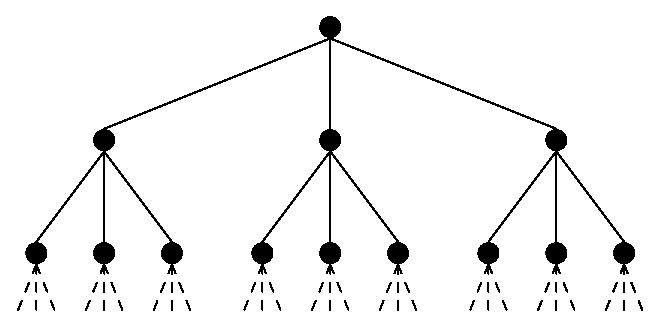
\includegraphics[height=75px]{ChapterSeqSer/Figures/PopulationModel}
	\end{wrapfigure}

Suppose we have a mama critter who is pregnant with three baby critters.  Each generation, each critter will give birth to three  new critters.  Let's find a formula for the number of descendants up to and including $n$ generations of descendants.  To get started, we make a table listing the population each generation.

\begin{center}
\begin{tabular}{|c|c|c|c|} \hline
Year & Summation & Description & Total \\ \hline & & & \\
0 & 1 & Just the mama & 1 \\ & & & \\
1 & 1+3 & The mama and her three children & 4 \\ & & & \\
2 & $1+3+3^2$ & The mama, three children, and nine grandchildren & 13  \\  & & & \\ 
3 & $1+3+3^2+3^3$ & All previous plus twenty-seven great-grandchildren & 40  \\  
\vdots & \vdots & \vdots & \vdots \\
$N$ & $\sum_{n=0}^N 3^n$ & $N$ generations of descendants & GSF \\ & & & \\
\hline
\end{tabular}
\end{center}
where GSF stands for Geometric Series Formula.  We now use it to evaluate the general summation.

$$\sum_{n=0}^N 3^n=\left(1\right)\left(\frac{1-3^{N+1}}{1-3}\right)=\left(\frac{1-3^{N+1}}{-2}\right)=\frac{1}{2}\left(3^{N+1}-1\right)$$
Thus, the model predicts that after $N$ generations, there are $\frac{1}{2}\left(3^{N+1}-1\right)$ total critters in the family tree.
\end{example}

\begin{exercise}{Meeting Critter-ia for a Geometric Series \Coffeecup}
\begin{itemize}
\item In the above example, why was it valid to use the Geometric Series Formula? 
\vspace*{.3in}
\item In the above example, plug in $N=0,1,2$, and 3 into the formula $\frac{1}{2}\left(3^{N+1}-1\right)$ and verify that it produces the correct totals.
\vspace*{.5in}
\item The above example demonstrates that the quantity $3^{N+1}-1$ is always divisible by 2.  Why is this the case?
\vspace*{.5in}
\end{itemize}
\end{exercise}

Economists often use Geometric Series when studying economic activity.  The exercise below is related to the idea of the \emph{velocity of money}, a measurement of how quickly money gets re-spent as it is received.  

\begin{exercise}{Velocity of Money \Coffeecup \Coffeecup } Let us a consider a simple model of income and spending.  People on average spend 80\% of what income they receive.  For example, say a contractor earns \$100,000 for a building job.  He then spends 80\% of this on a fancy automobile. Collectively, the car salesman, dealership, and auto manufacturer receive \$80,000.  They in turn go spend 80\% of that \$80,000 on going out to dinner, reinvestment in their business, or other goods and services that are then received as income by others.  Thus, these others will receive \$64,000 which they in turn will again go out and spend 80\% of.  


Suppose also that on average, money changes hands roughly once a month.  That is, there is a one-month delay between receiving money as income and going out to spend it. 


The government invests \$5 billion in public infrastructure.  How much total economic activity is actually generated by this investment in one year? Use the Geometric Series Formula to evaluate your answer!

\vspace*{1in}
\AnswerKeyEntry{$\$5 \text{ billion }\cdot\frac{1-0.8^{13}}{1-0.8}\approx \$23.6 \text{ billion}$}
\end{exercise}

Here is an example that will initially look out of place in this section.  We will later see why this is in fact geometric series in disguise!  

\begin{exercise}{\fibonacci{Partial Sums} of Fibonacci Numbers \Coffeecup \Coffeecup \Coffeecup}\label{Lieonacci}
Recall $F_n$, the sequence of Fibonacci numbers. 
\begin{itemize} 
\item Compute the following quantities:
\begin{align*}
F_0&=\\
F_0+F_1&=\\
F_0+F_1+F_2&=\\
F_0+F_1+F_2+F_3&=\\
F_0+F_1+F_2+F_3+F_4&=\\
F_0+F_1+F_2+F_3+F_4+F_5&=\\
F_0+F_1+F_2+F_3+F_4+F_5+F_6&=
\end{align*}

\item Explain why $F_0+F_1+\cdots+F_N$ cannot be evaluated by directly applying the Arithmetic or Geometric Series Formula.

\vspace*{.5in}

\item Do you notice any patterns in the sums above?  In particular, see if you can express the sum of Fibonacci numbers $ \sum_{i=0}^n F_i$ in terms of just a single Fibonacci number.

\vspace*{1in}
\end{itemize}
\AnswerKeyEntry{Try to notice how the summations relate to the very next Fibonacci number, the first one not being summed.}
\end{exercise}
We don't have the tools at the moment to prove that formula is correct, but we will revisit this example in Chapter \ref{FigAndGnocchiNumbers}.
